\documentclass[12pt]{beamer}

\usepackage{pgfpages}

% These slides also contain speaker notes. You can print just the slides,
% just the notes, or both, depending on the setting below. Comment out the want
% you want.

\setbeameroption{hide notes} % Only slides
%\setbeameroption{show only notes} % Only notes
%\setbeameroption{show notes on second screen=right} % Both

% To give a presentation with the Skim reader (http://skim-app.sourceforge.net) on OSX so
% that you see the notes on your laptop and the slides on the projector, do the following:
% 
% 1. Generate just the presentation (hide notes) and save to slides.pdf
% 2. Generate onlt the notes (show only nodes) and save to notes.pdf
% 3. With Skim open both slides.pdf and notes.pdf
% 4. Click on slides.pdf to bring it to front.
% 5. In Skim, under "View -> Presentation Option -> Synhcronized Noted Document"
%    select notes.pdf.
% 6. Now as you move around in slides.pdf the notes.pdf file will follow you.
% 7. Arrange windows so that notes.pdf is in full screen mode on your laptop
%    and slides.pdf is in presentation mode on the projector.

% Give a slight yellow tint to the notes page
\setbeamertemplate{note page}{\pagecolor{yellow!5}\insertnote}\usepackage{palatino}

\title{Sinusfunktion, Cosinusfunktion}
\author{Elias Leitinger}
\date{\small Planet Earth}

\begin{document}

\begin{frame}
  \titlepage

  \note[item]{Introduction etc.}
\end{frame}

\begin{frame}
  \frametitle{Grundkompetenzen}
  \begin{itemize}
  \item FA 6.1: grafisch oder durch eine Gleichung gegebene Zusammenhänge der Art $f(x)= a*\sin(b*x)$
als allgemeine Sinusfunktion erkennen beziehungsweise betrachten können; zwischen diesen Darstellungen
wechseln können
  \item FA 6.2: aus Graphen und Gleichungen von allgemeinen Sinusfunktionen Werte(paare) ermitteln
und im Kontext deuten können.
  \item FA 6.3: die Wirkung der Parameter a und b kennen und die Parameter im Kontext deuten können
  \item FA 6.4: Periodizität als charakteristische Eigenschaft kennen und im Kontext deuten können
  \item FA 6.5: wissen, dass $\cos(x) = \sin(x+\frac{\pi}{2})$
  \item FA 6.6: wissen, dass gilt: $[\sin(x)]' = \cos(x)$, $[\cos(x)]' = -\sin(x)$
  \end{itemize}
  

\end{frame}

\begin{frame}
  \frametitle{Parameter der allgemeinen Sinusfunktion $f(x)=a*\sin(b*x)$}
  %\begin·{itemize}
  %  \item a staucht oder streckt die Funktion in y-Richtung
  %  \item b staucht oder streckt die Funktion entlang der x-Achse
  %\end{itemize}
  \begin{itemize}
    \item a staucht oder streckt die Funktion in y-Richtung
    \item b staucht oder streckt die Funktion entlang der x-Achse
  \end{itemize}
  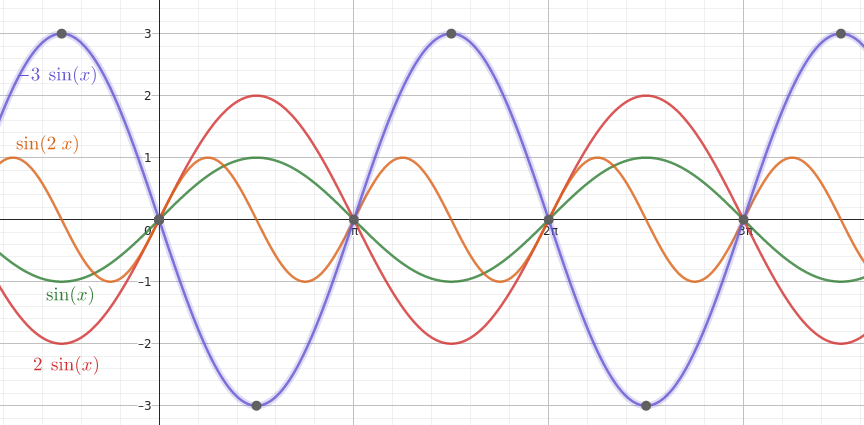
\includegraphics[width=\textwidth]{sin}
  \note[item]{a legt die Schwankungsbreite fest → negativ => verkehtrt}
  \note[item]{b bestimmt wie häufig die Schwankung abläuft → Periodenlänge}
\end{frame}
\begin{frame}
  \frametitle{Periodizität}
  \begin{itemize}
    \item beschreibt, wie häufig etwas in einem Intervall passiert
    \item wird bei sinusfunktionen durch den Parameter b bestimmt
    \item wird durch Periodenlänge p angegeben
  \end{itemize}
\end{frame}
\begin{frame}
  \frametitle{Wirkung der Parameter}
  \begin{itemize}
    \item $|a|$ gibt an, welchen wert die Maxiumumstellen annehmen
    \item wenn $a < 0$, dann ist die erste Extremstelle nach $x = 0$ eine Minimumstelle
    \item wenn $a > 0$, dann ist die erste Extremstelle nach $x = 0$ eine Maximumstelle
    \item wenn $b = 1$, dann ist die Periodizität $p = 2\pi$
    \item wenn $b \neq 1$, dann beträgt die Periodizität $p = \frac{2\pi}{b}$
  \end{itemize}
\end{frame}
\begin{frame}
  \frametitle{Werte ermitteln und im Kontext deuten}
  \begin{itemize}
    \item Zur Modellierung von Wellen oder sich wiederholenden Bewegungen (Federpendel) → Zeit als Parameter
    \item Zum Modellieren von Bewegung auf Kreisbahn (Radius: Parameter a; Umlaufzeit: Zeit, die für ganze Periode der Sinusfunktion benötigt wird)
    \item Ermittlung von Extremstellen und Nullstellen aus gegebenen Funktionen bei wiederholten Handlungen (Atmung)
  \end{itemize}
\end{frame}
\begin{frame}
  \frametitle{Lösungen}
  \begin{itemize}
    \item $a = 2, b = 1.5$
    \item radius: 4dm; Umlaufzeit: 6s
    \item $\frac{2\pi}{b}$
  \end{itemize}
\end{frame}

\end{document}